\section{Volume exploration space}
\label{sect:volume-exploration-space}

Figure~\ref{fig:tf-design-example} illustrates the TF design interface, a 2D scatter plot where each circle represents a pivot selected by SSS. The positions from FastMap determine the points' coordinates. Each pivot is a central point of a cluster, with its circle radius proportional to the number of voxels it represents, normalized logarithmically.

\begin{figure}[htb!]
    \centering
    \subfloat[Initial transfer function specification (semi-automatic generated).\label{subfig:tf-design-example-generated}]{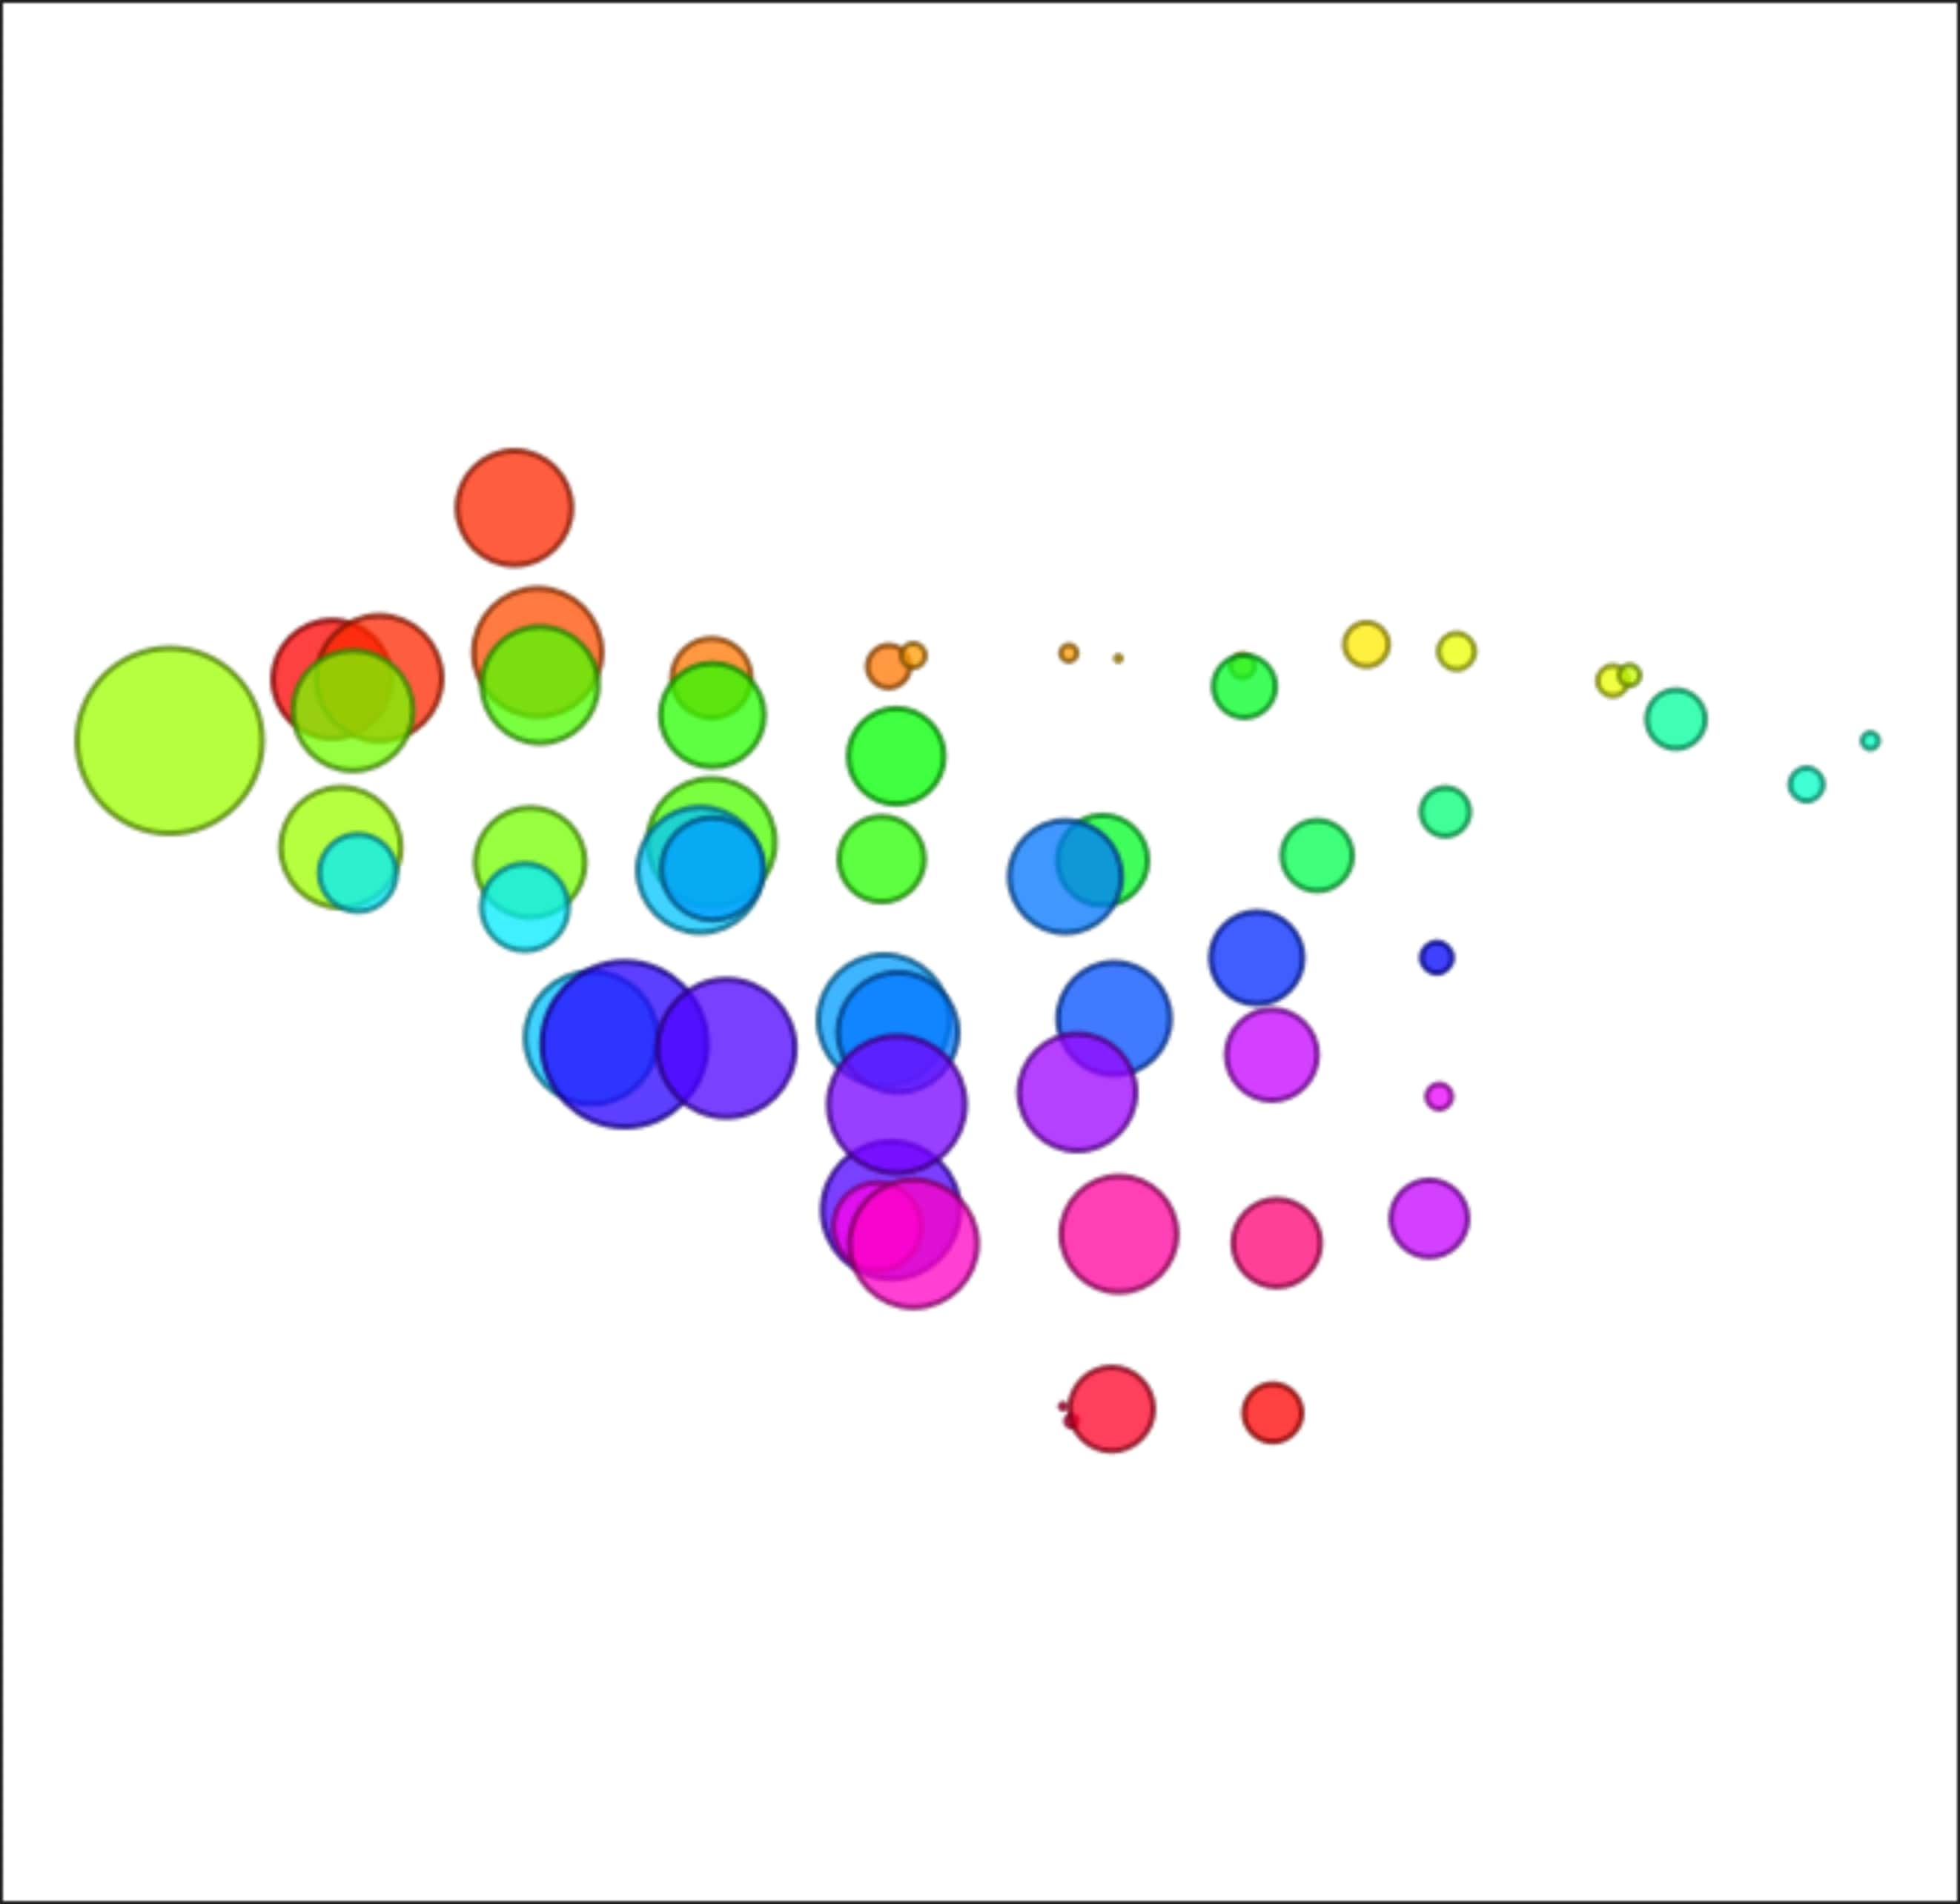
\includegraphics[width=0.6\columnwidth]{figs/tf-design-interface-a.jpg}}
    \hfill
    \subfloat[Fine-tune material classification after user adjustment.\label{subfig:tf-design-example-user}]{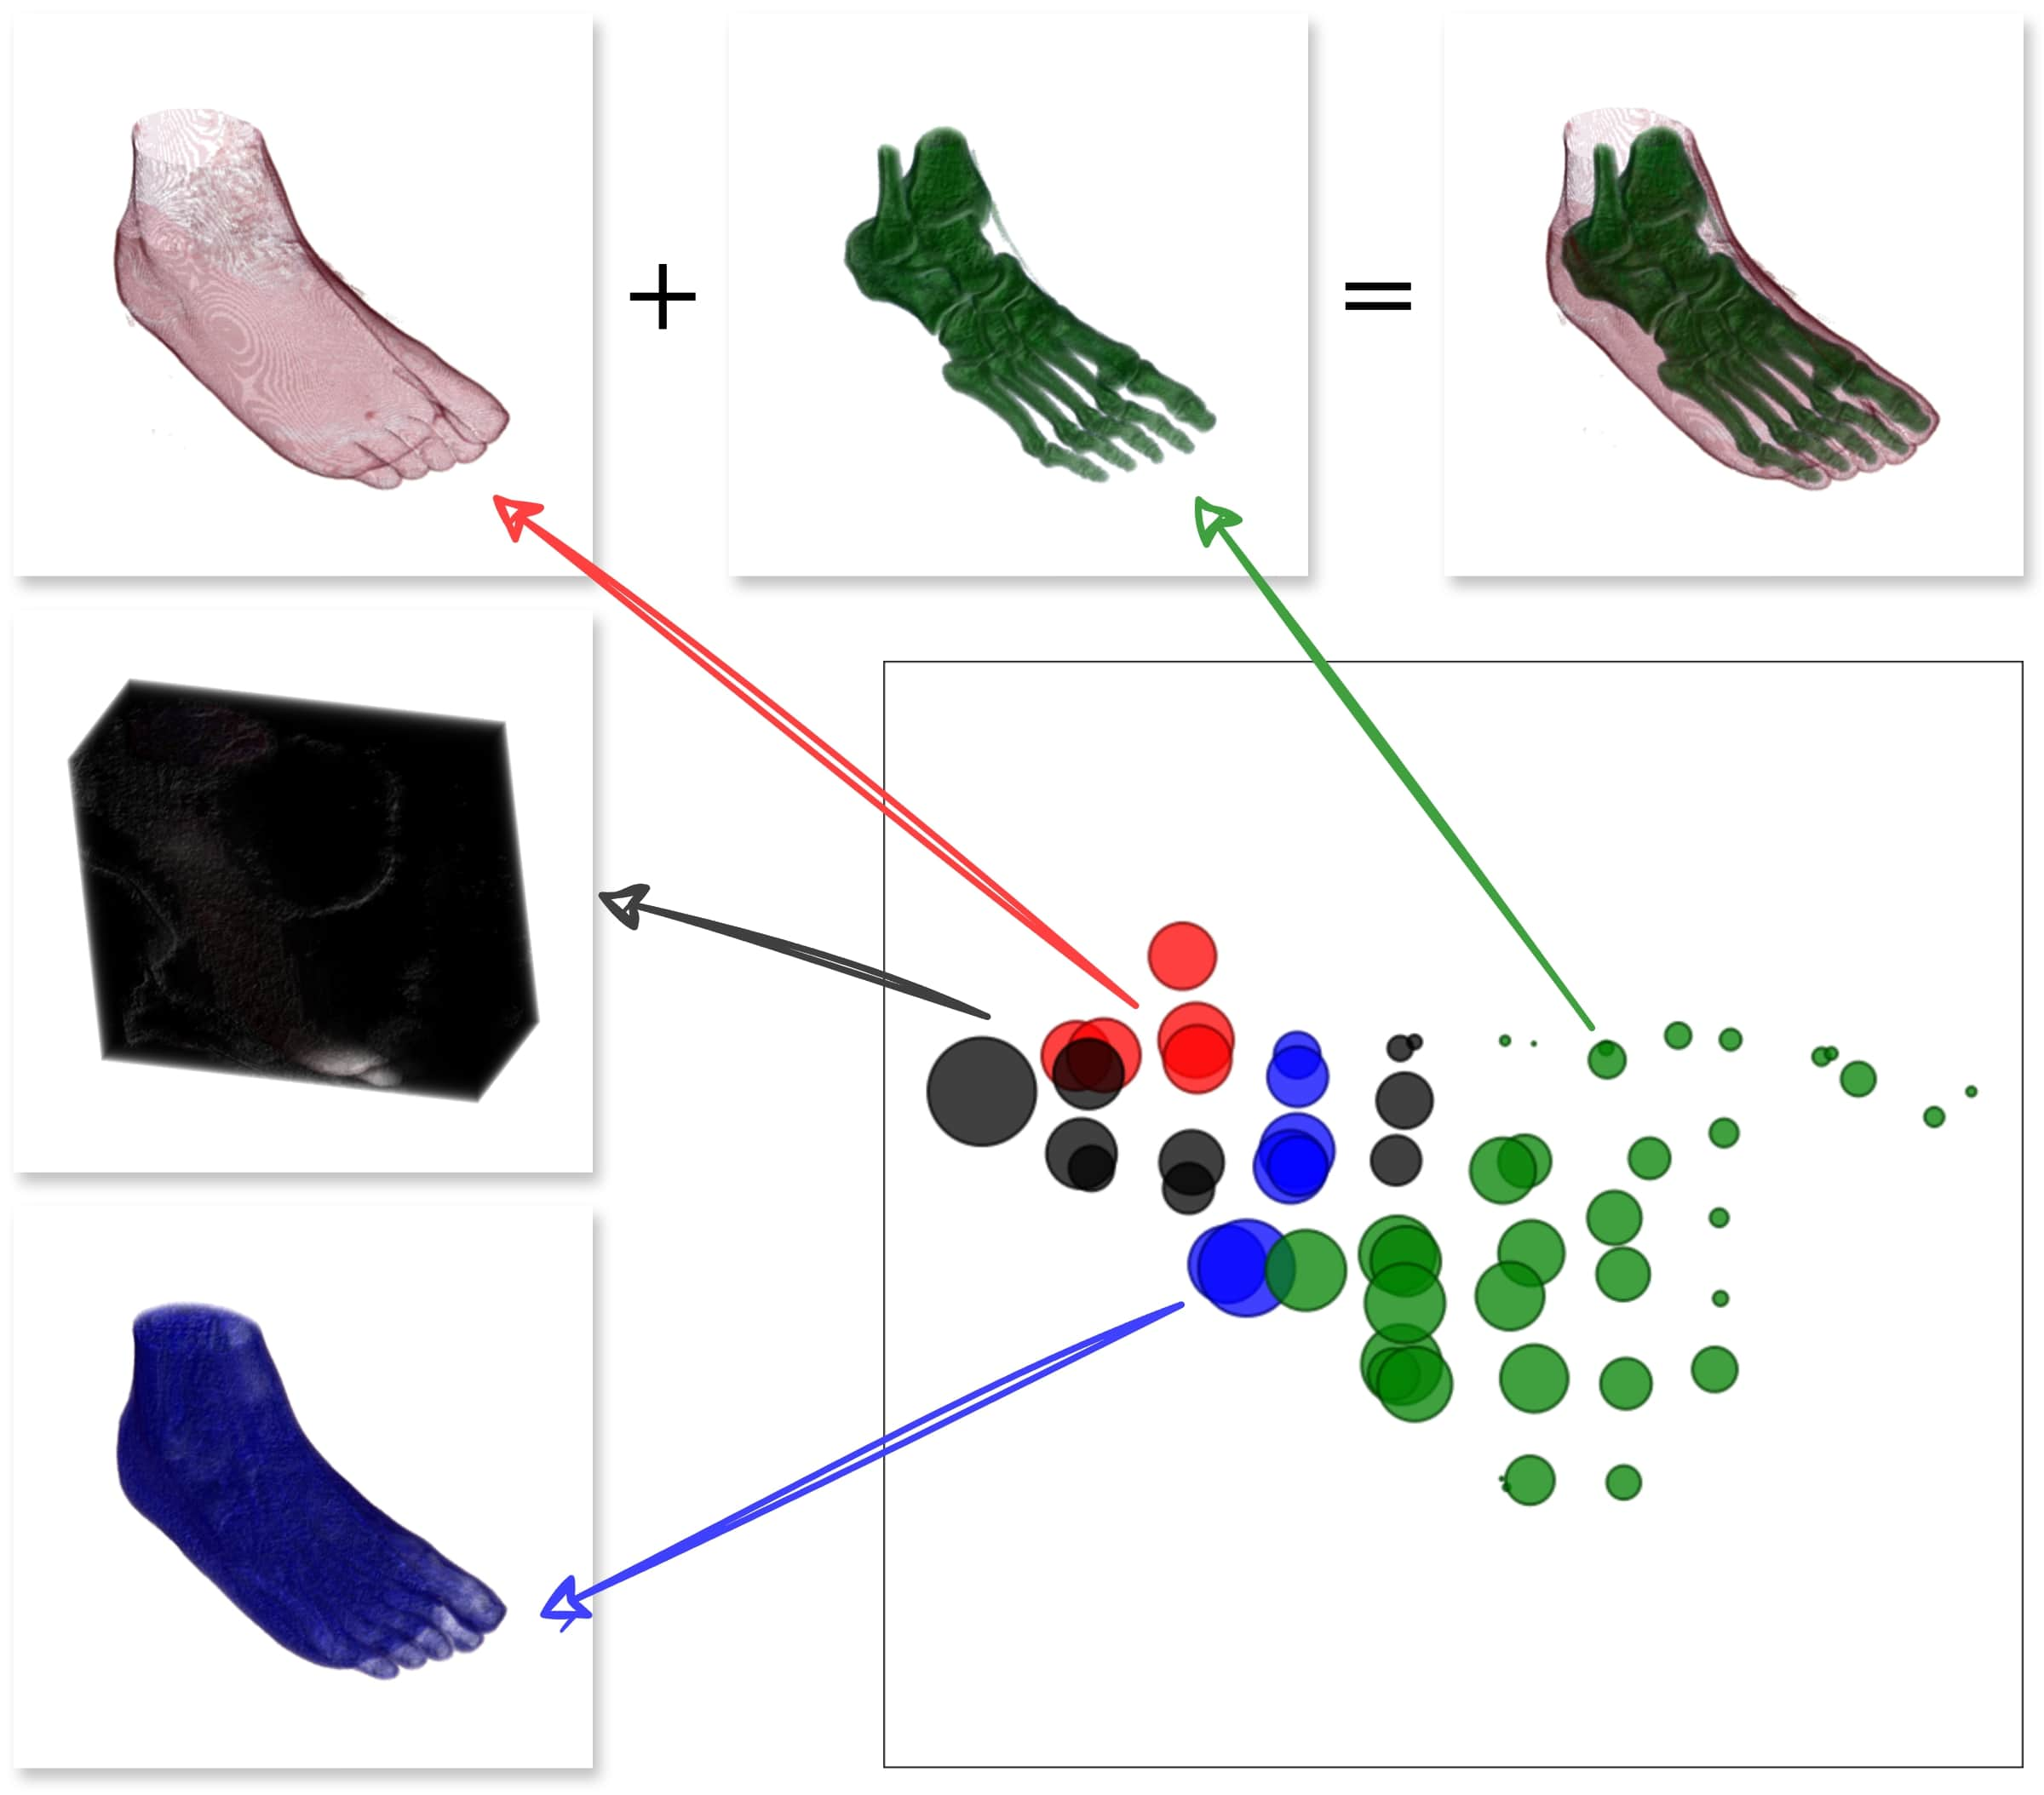
\includegraphics[width=0.6\columnwidth]{figs/tf-design-interface-b.jpg}}
    \caption{Transfer function design interface and volume exploration space of a right male foot dataset.}
    \label{fig:tf-design-example}
\end{figure}

Our method generates an initial TF specification using a predefined opacity and a rainbow color scale, assigning a unique color per cluster.

Users adjust the TF following the WYSIWYG principle: pivot color and opacity map directly to their associated voxels according to clustering. Both selected and unselected elements can be customized.

Volume exploration occurs through pivot selection. The system dynamically increases the opacity of selected pivots and decreases that of others. Users can make arbitrary selections, save them as groups, and interact with pivots, clusters, or groups as selectable entities.

Iterative selection of nearby elements aids identifying volume details. FastMap and DBSCAN naturally cluster similar instances spatially, simplifying this process.

Our approach automates material classification by assuming each cluster or pivot represents a relevant item. If unsatisfied, users may select/deselect elements or adjust parameters:

\begin{itemize}
    \item input volume data,
    \item DBSCAN parameters $\varepsilon$ and $minPts$,
    \item SSS distance factor $\alpha$.
\end{itemize}
